La technique ne change pas: nous allons restreindre la recherche à des polygones de plus en plus particuliers. Cette dernière section nous poussera à un peu plus de technicité.


% ----------------------- %


\begin{defi}
	Un \og \emph{$n$-gone} \fg\ désigne un polygone à $n$ côtés avec $n \geq 3$.
\end{defi}


\begin{defi}
	Un \og \emph{$n$-isogone} \fg\ désigne un $n$-gone dont tous les côtés sont de mesure égale.
\end{defi}


% ----------------------- %


\begin{fact}\label{conv-poly}
	Si un $n$-gone $\setproba{P}$, de périmètre fixé $p$, n'est pas convexe, alors on peut construire à partir de $\setproba{P}$ un $n$-gone convexe $\setproba{P}^{\,\prime}$ tel que $\perim{\setproba{P}^{\,\prime}} = p$ et $\area{\setproba{P}^{\,\prime}} > \area{\setproba{P}}$.
\end{fact}


\begin{proof}
	Ici, il ne faut pas être expéditif en indiquant que la preuve du fait \ref{quadri} se généralise sans aucun souci.
	En effet, avec $n > 4$, nous pouvons avoir plusieurs points de non-convexité, et les éliminer comme nous l'avons fait pour le quadrilatère n'est pas immédiat:
	dans la figure suivante, l'élimination des deux points de non convexité $G$ et $E$ de l'heptagone $ABCDEFG$ nous amène à un nouvel heptagone $ABCDE^{\,\prime}FG^{\,\prime}$ ayant lui aussi deux points de non-convexité $F$ et $D$!
	Donc, rien n'empêche, a priori, d'avoir une suite de constructions n'aboutissant jamais à un heptagone convexe de même périmètre que celui de $ABCDEFG$, et d'aire strictement supérieure à celle de $ABCDEFG$.

	\begin{center}
		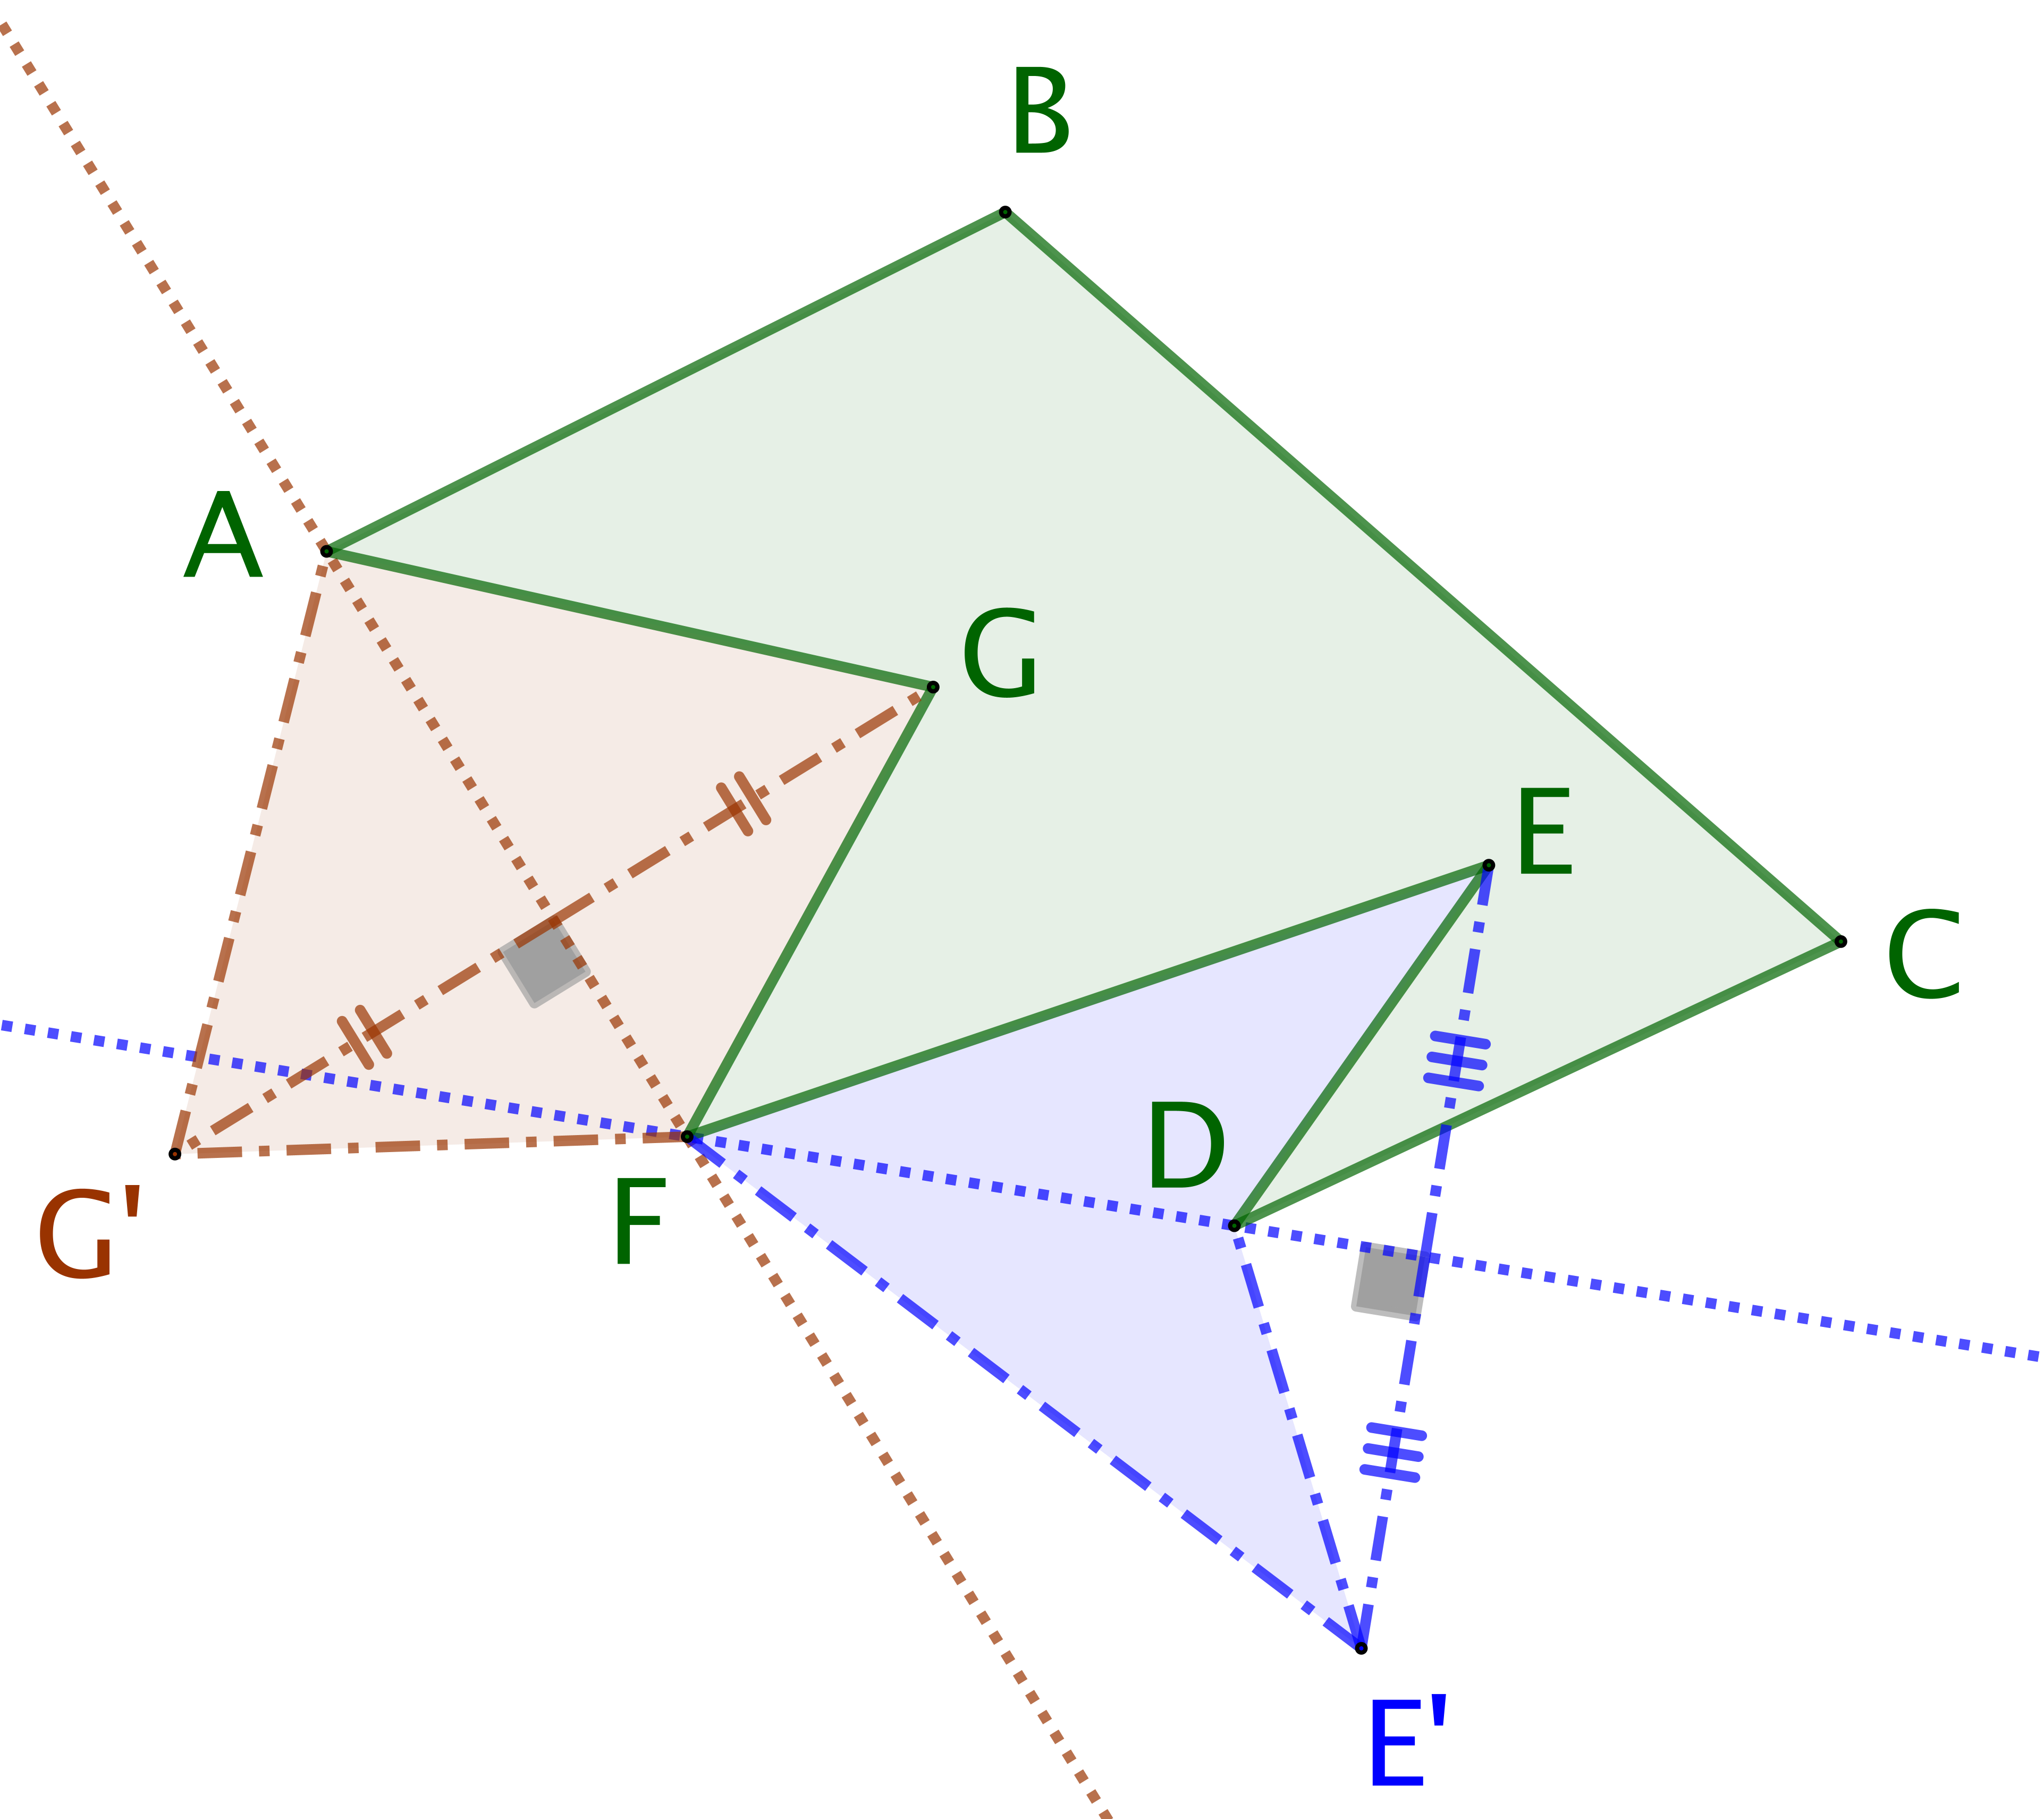
\includegraphics[scale=.4]{content/polygon/polygon-non-convex-trap.png}
	\end{center}
	

	La solution est \og \emph{simple} \fg\ : il faut être moins exigeant. 
	En effet, pour un $n$-gone non convexe $\setproba{P}$, de périmètre fixé $p$, nous allons considérer son enveloppe convexe $\setproba{P}^{\,\prime}$ qui est le plus petit polygone convexe contenant $\setproba{P}$ (pas de panique, on en reparle plus rigoureusement juste après). 
	Par exemple, dans la figure suivante, l'enveloppe convexe de l'ennéagone $ABCDEFGHI$ est le pentagone $ABDEG$ 
	qui vérifie
	$\perim{ABDEG} < \perim{ABCDEFGHI}$, ainsi que
	$\area{ABDEG} > \area{ABCDEFGHI}$.
	Une homothétie de rapport
	$r = \frac{\perim{ABCDEFGHI}}{\perim{ABDEG}}$
	nous donne finalement un pentagone convexe de périmètre $\perim{ABCDEFGHI}$, et d'aire strictement supérieure à $\area{ABCDEFGHI}$.
	Voilà! Il ne reste plus qu'à démontrer cela proprement, et ceci pour le cas général.
	
	\begin{center}
		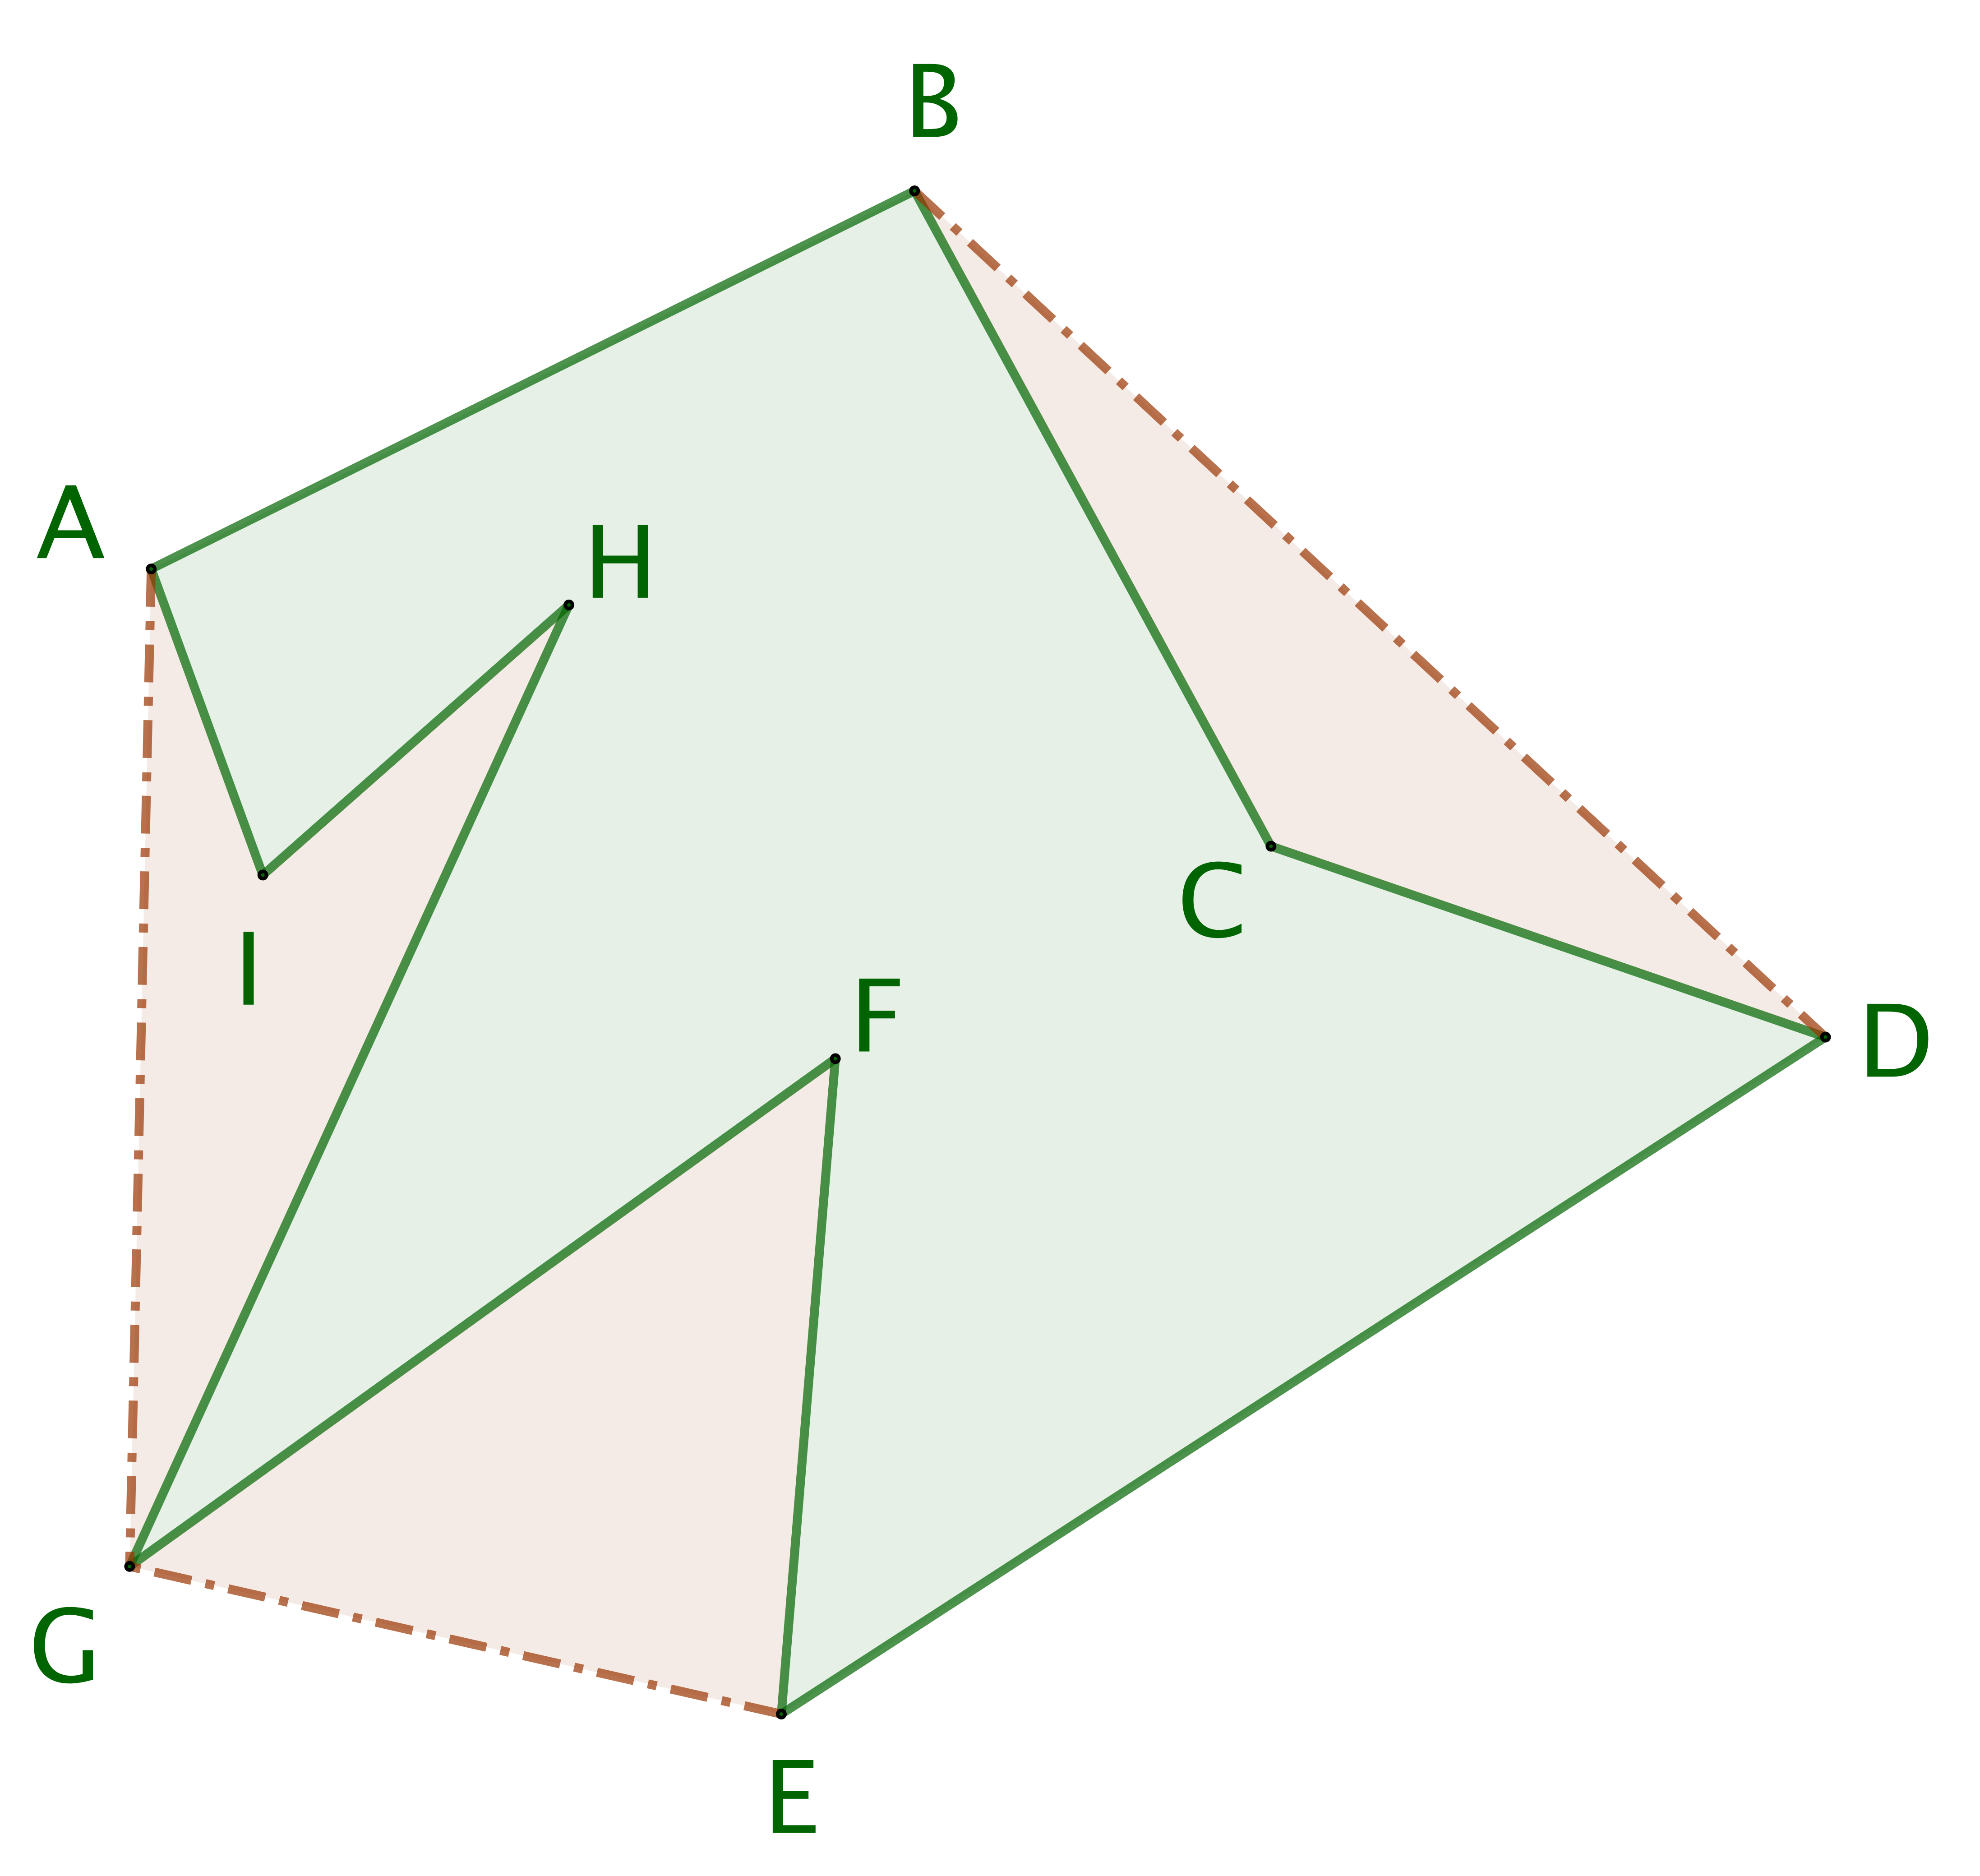
\includegraphics[scale=.4]{content/polygon/polygon-non-convex.png}
	\end{center}
	
	
	Voici un moyen simple de construire l'envelope convexe d'un $n$-gone qui nous donnera aussi au passage ce que l'on souhaite sur les périmètres et les aires.
	%
	\begin{itemize}
		\item XXX

		\item XXX

		\item XXX

		\item XXX
	\end{itemize}
\end{proof}


% ----------------------- %


\begin{fact}\label{iso-poly}
	Si un $n$-gone convexe $\setproba{P}$, de périmètre fixé $p$, n'est pas un $n$-isogone, alors on peut construire à partir de $\setproba{P}$ un $n$-isogone convexe $\setproba{P}^{\,\prime}$ tel que $\perim{\setproba{P}^{\,\prime}} = p$ et $\area{\setproba{P}^{\,\prime}} > \area{\setproba{P}}$.
\end{fact}


\begin{proof}
	XXX
\end{proof}


% ----------------------- %


Les faits \ref{conv-poly} et \ref{iso-poly} précédents permettent de se restreindre au cas des $n$-isogones convexes. Ceci nous amène au beau résultat suivant.

\begin{fact}\label{reg-poly}
	Si un $n$-isogone convexe $\setproba{P}$ de périmètre fixé $p$ possède au moins deux angles de mesures différentes, alors on peut construire à partir de $\setproba{P}$ un $n$-gone régulier $\setproba{P}^{\,\prime}$ tel que $\perim{\setproba{P}^{\,\prime}} = p$ et $\area{\setproba{P}^{\,\prime}} > \area{\setproba{P}}$.
\end{fact}


\begin{proof}
	XXX
\end{proof}


% ----------------------- %


\begin{fact}
	Soit $n \in \NN_{\geq3}$ un naturel fixé.
	Considérons tous les $n$-gones de périmètre fixé $p$. Parmi tous ces $n$-gones, un seul est d'aire maximale, c'est le $n$-gone régulier.
\end{fact}


\begin{proof}
	Tout a déjà été dit, car d'après les faits ci-dessus, un $n$-gone $\setproba{P}$ non régulier ne peut pas maximiser son aire à périmètre fixé, et par conséquent seul le $n$-gone régulier maximise l'aire à périmètre fixé. Chapeau bas, géométrie...
\end{proof}
